
\begin{frame}[t,allowframebreaks]{Capacity -}

    We can affect the tendency of a \gls{ml} model for 
    \index{underfitting}\gls{underfitting} or 
    \index{overfitting}\gls{overfitting},
    by adjusting its 
    \index{capacity}\gls{capacity}.\\

    \vspace{0.2cm}

    The \gls{capacity} of a model is its 
    {\bf ability to describe a broad variety of data-generating processes}.

    \vspace{0.2cm}

    \begin{itemize}
        \item 
        {\bf Models with low capacity, 
        will struggle capturing all the details} 
        of the training data and providing a satisfactory fit.\\
        % \begin{blockexample}{}
        %     \small
        %     For example, imagine using a linear model $\hat{y} = b+wx$
        %     to fit data sampled from a data-generating process with a 
        %     probability distribution that is quadratic in $x$.
        % \end{blockexample}
        \item 
        {\bf Models with high capacity 
        can memorize unimportant features} of the data
        that do not serve the purpose of model Generalisation.
        % \begin{blockexample}{}
        %     \small
        %     For example, imagine using a 10$^{th}$ order polynomial to
        %     to fit noisy data sampled from a data-generating process with a 
        %     probability distribution that is linear in $x$.
        % \end{blockexample}
    \end{itemize}

    \vspace{0.2cm}

    Occam's razor (the `law of parsimony')
    \cite{Wikipedia:OccamRazor} is a good guiding principle:
    Amongst competing hypotheses that describe the data equally well,
    chose the simples one.\\

    \vspace{0.2cm}

    While simpler models are likely to generalise better,
    we still need a sufficiently complex model to achieve low training error.

    \framebreak

    %
    %

    A central task in \gls{ml} is to {\bf match the capacity of the model
    to the complexity of its task and to the amount of available data.}\\

    \vspace{0.1cm}

    \begin{center}
        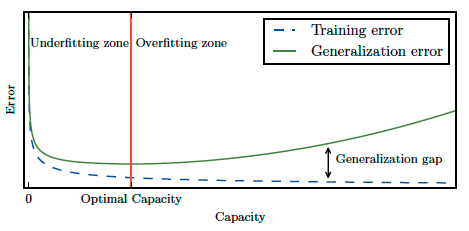
\includegraphics[width=0.90\textwidth]
            {./images/training_issues/goodfellow17_error_vs_capacity_1.png}\\
        {\tiny 
            Illustrating the relationship between error and capacity.\\
            \color{col:attribution} 
            Schematic reproduced from p. 112 of \cite{Goodfellow:2017MITDL}.\\
        }
    \end{center}

    \framebreak

    %
    %

    There are several ways to affect the capacity of a model.


\end{frame}
